\chapter{Plastic Materials}


%\section{Phenomenological Features of the Elastic-Plastic  Response}
%
%
%The fundamental characteristics of the elastic-plastic behavior of polycrystalline metals can be illustrated through the stress-strain curve obtained from a uniaxial tensile test. In such an experiment, a cylindrical sample with initial length $L_0$ and cross-sectional area $A_0$ is stretched to a new length $L$, resulting in an axial force $P$. The \emph{engineering stress} (or Piola stress), defined with respect to the undeformed area, is given by
%\[
%s = \frac{P}{A_0}.
%\]
%
%If $\lambda = L / L_0$ denotes the axial stretch ratio, then the associated \emph{engineering strain} is defined as
%\[
%e = \lambda - 1.
%\]
%
%\begin{figure}
%	\centering
%	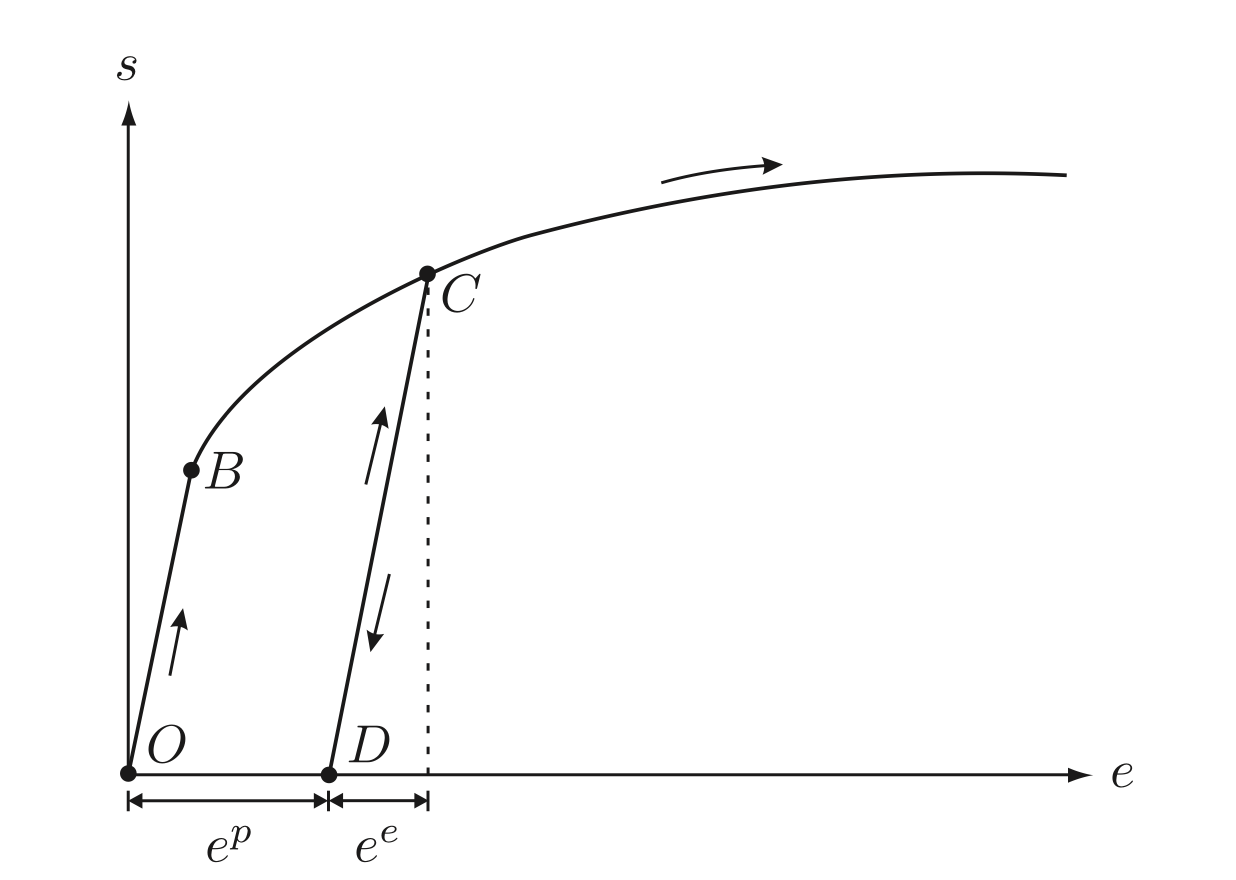
\includegraphics[width=0.6\linewidth]{figure/problema_elastico/plastic}
%	\caption{Schematic of an engineering stress-strain curve for a metallic material.}
%	\label{fig:plastic}
%\end{figure}
%
%A typical engineering stress versus strain curve for metals is presented in Fig. \ref{fig:plastic}; it shows an initial linear segment $OB$, representing elastic behavior. Reversing the loading path within this region results in a retraced path along the same line, indicating reversible deformation. The point $B$ marks the limit of linearity, known as the \emph{elastic limit}, and the corresponding stress is referred to as the \emph{yield strength}.
%
%Beyond the yield point, the curve departs from linearity, and stress continues to rise with increasing strain. This region corresponds to \emph{strain hardening}, where the material supports higher loads despite a decrease in cross-sectional area. This segment is often called the \emph{hardening curve}.
%
%If unloading begins from a point $C$ beyond the elastic regime, the stress does not follow the original loading path. Instead, the material unloads elastically along a different path $CD$, characterized by partial recovery of the deformation. The strain recovered during this stage is the \emph{elastic strain} $e^e$, while the remaining permanent strain is the \emph{plastic strain} $e^p$. A subsequent reloading from point $D$ typically returns along the unloading path, eventually rejoining the hardening curve at $C$, after which further loading continues along the existing hardening trajectory.
%
%In addition to engineering stress, one may also consider the \emph{true stress} (or Cauchy stress), which accounts for the instantaneous cross-sectional area $A$:
%\[
%\sigma = \frac{P}{A}.
%\]
%
%In addition to engineering strain, the \emph{true strain} (also referred to as logarithmic strain) is defined by the relation
%\[
%\epsilon = \ln \lambda.
%\]
%
%To determine the true stress during a tensile test, one must measure both the applied force $P$ and the instantaneous cross-sectional area $A$ of the specimen. Since concurrent measurements of elongation and lateral contraction are uncommon in typical tests, it is standard to assume that the plastic deformation of metals occurs at nearly constant volume (incompressibility). While elastic deformation involves volume changes, these are negligible compared to plastic effects.
%
%Under this assumption, the volume of the specimen remains approximately constant:
%\[
%A L \approx A_0 L_0.
%\]
%Using this, the true stress $\sigma$ and true strain $\epsilon$ can be related to engineering measures as:
%\[
%\sigma = \frac{P}{A} = \frac{P}{A_0} \cdot \frac{L}{L_0} = s(1 + e), \qquad \epsilon = \ln(1 + e).
%\]
%
%These expressions enable conversion from engineering stress and strain to their true counterparts.
%
%\vspace{1em}
%
%When true stress-strain curves from tension and compression tests are compared—both performed at ambient conditions—it is often observed that they nearly coincide for most metals. This indicates that the intrinsic plastic behavior of the material is independent of the type of loading. Conversely, engineering stress-strain curves for tension and compression often differ significantly due to the evolving geometry during deformation. Consequently, the \textit{true stress-strain curve is generally accepted as the most accurate representation of the material’s intrinsic plastic behavior}.
%
%\vspace{1em}
%\begin{figure}
%	\centering
%	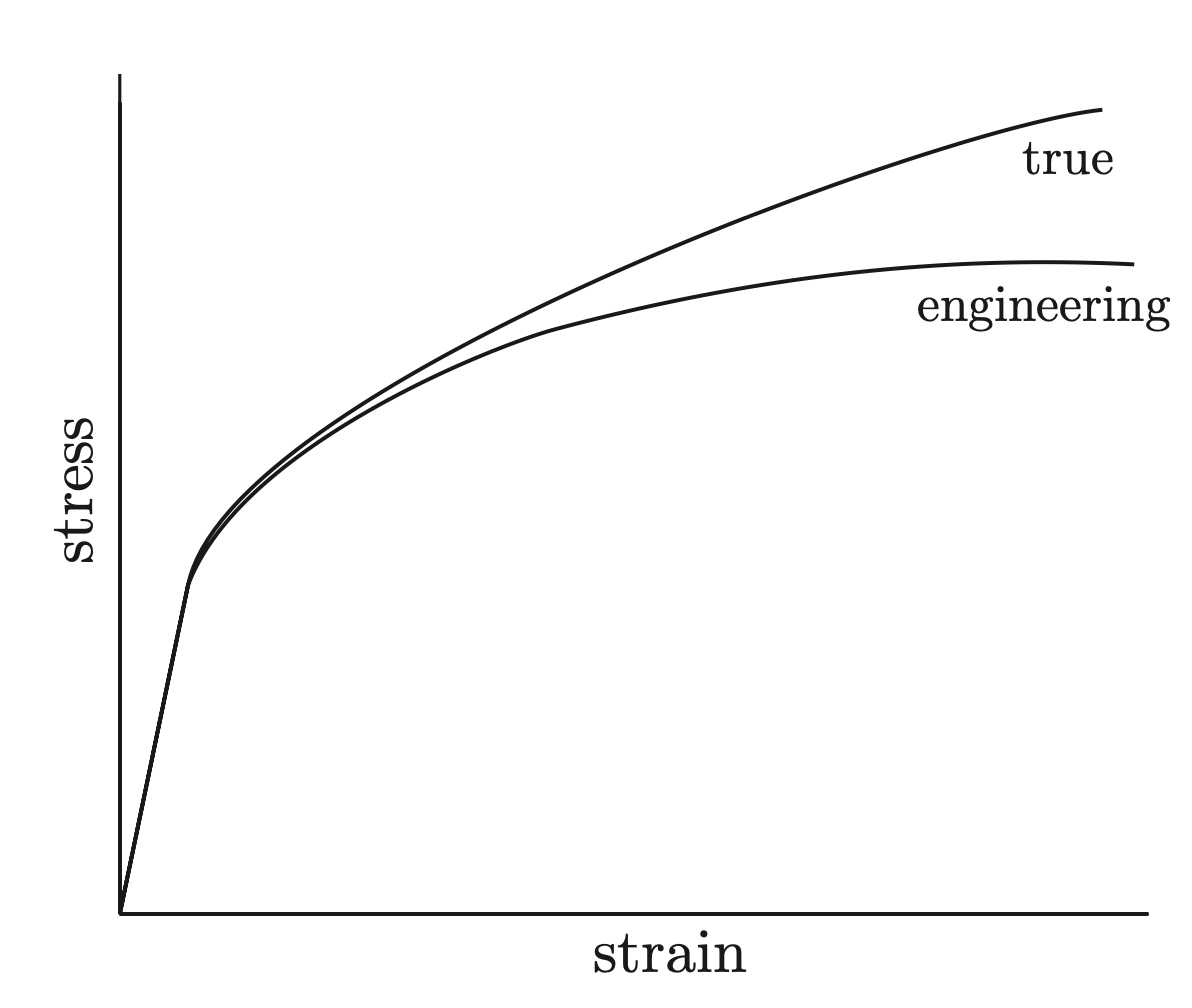
\includegraphics[width=0.5\linewidth]{figure/problema_elastico/plastic1}
%	\caption{Comparison of a true stress-strain curve with the corresponding engineering
%		stress-strain curve.}
%	\label{fig:plastic1}
%\end{figure}
%
%The mechanical behavior of metals under cyclic loading differs substantially from that under monotonic loading. One prominent feature observed is the \emph{Bauschinger effect}, initially described by Bauschinger in 1886. This effect refers to the reduction in yield stress upon load reversal: a metal specimen that has been plastically stretched shows a diminished resistance when subsequently compressed. 
%
%
%
%A schematic of such reversed-loading behavior is illustrated in Figure \ref{fig:plastic1}, where the solid line depicts the true stress-strain path of a sample first loaded in tension, followed by compression.
%
%\subsection*{74.1 Isotropic and Kinematic Strain-Hardening}
%
%As is clear from our brief discussion of the phenomenology of the stress-strain response, the deformation of metals beyond the elastic limit is quite complicated. In this subsection, we discuss some idealizations of strain-hardening that are frequently used in theories of plasticity.
%
%A simple idealization of actual material response, referred to as \textbf{isotropic hardening}, accounts for strain-hardening but approximates the hardening by a straight line, neglects the Bauschinger effect, and assumes that after reversal of deformation from any level of strain in the plastic regime, the magnitude of the flow stress upon which reverse yielding begins has the same value as the flow stress from which the unloading was initiated. The stress-strain response corresponding to isotropic hardening is shown schematically in Figure 74.4(a).
%
%Let the stress level from which reversed deformation is initiated be denoted by $\sigma_f$, and denote the stress at which the stress-strain curve in compression begins to deviate from linearity by $\sigma_r < 0$. The closed interval $[\sigma_r, \sigma_f]$ is called the \emph{elastic range}, and its endpoints $\{\sigma_r, \sigma_f\}$ are called the \emph{yield set}. Let $Y$, with initial value $Y_0$, denote the \emph{flow resistance} (a material property) of the material. The initial elastic range then has
%\[
%\sigma_r = -Y_0, \quad \sigma_f = Y_0,
%\]
%and, during subsequent plastic deformation along the hardening curve, the deformation resistance increases linearly from $Y_0$ to $Y$ due to strain-hardening, and the new elastic range becomes
%\[
%\sigma_r = -Y, \quad \sigma_f = Y.
%\]
%For such an idealized response of an elastic-plastic material, the magnitude of the stress $\sigma$ in this elastic range is bounded with the restriction
%\[
%|\sigma| \leq Y,
%\]
%generally referred to as a \emph{yield condition}, with plastic flow possible when $|\sigma| = Y$.
%
%Isotropic strain-hardening is an idealization of the actual hardening behavior of metals; in particular, it does not account for the Bauschinger effect. An alternative simple model for strain-hardening that accounts for this phenomenon is referred to as \textbf{kinematic hardening}. The stress-strain response for a material with linear kinematic hardening is shown in Figure 74.4(b): the initial flow resistance is $Y_0$; upon deformation in tension into the plastic regime, the stress increases linearly to $\sigma_f$, and, upon reversal of deformation, the material starts to plastically flow at a stress level $\sigma_r < 0$ and thereafter again continues to harden linearly. The magnitude $|\sigma_r|$ of the stress at which plastic flow recommences upon load reversal is smaller than that of $\sigma_f$, at which the reversed loading event was initiated — which embodies the \emph{Bauschinger effect}. The asymmetry in the onset of yield upon reversal of loading in such a model arises because of the buildup of an internal stress called the \emph{backstress} and denoted by $\sigma_b$, whose magnitude is equal to
%\[
%\sigma_b = \frac{1}{2} (\sigma_f + \sigma_r).
%\]
%
%The term \emph{kinematic hardening} reflects the fact that the center of the \emph{elastic range} in stress space moves from an initial value of $\sigma = 0$ to a value of $\sigma = \sigma_b$, while the height of the elastic range remains constant at $2Y_0$. This is in contrast to isotropic hardening shown in Figure 74.4(a), where the \emph{elastic range} in stress space stays centered at $\sigma = 0$, while the height of the elastic range expands from $2Y_0$ to $2Y$ as the material strain-hardens. For the material with kinematic hardening described above, the stress obeys the yield condition
%\[
%|\sigma - \sigma_b| \leq Y_0.
%\]
%
%For many metals, the actual strain-hardening behavior — including the Bauschinger effect — may be approximated by a combination of nonlinear isotropic hardening and nonlinear kinematic hardening.



\section{Kinematical Assumptions}
Most theories of plasticity are grounded in a physical intuition that envisions a plastic solid as possessing an underlying microscopic structure---such as a crystal lattice---that can undergo stretching and rotation, along with the presence of defects like dislocations that can move within this structure. In what follows, we give mathematical form to this perspective by introducing a kinematical constitutive assumption that requires the displacement gradient to admit the specific decomposition:
\begin{equation}
\nabla\ub=\He+\Hp,
\end{equation}
where
\begin{enumerate}
	\item $\He$ is the \textit{elastic distortion}, representing stretch and rotation of the underlying microscopic structure;
	\item $\Hp$ is the \textit{plastic distortion}, representing the local deformation of material due to 	the formation and motion of dislocations through that structure.
\end{enumerate}

Let us introduce the \textit{elastic} and \textit{plastic strains}
\begin{equation}
	\Ee=\sym\He, \qquad \Ep=\sym\Hp,
\end{equation}and the \textit{elastic} and \textit{plastic rotations}
\begin{equation}
	\We=\skw\He, \qquad \Wp=\skw\Hp,
\end{equation}
so that
\begin{equation}
\Eb=\Ee+\Ep, \qquad \Wb=\We+\Wb.
\end{equation}
Finally, consistent with the general observation that the flow of dislocations
does not induce changes in volume, we assume that $\Hp$ is deviatoric, \textit{i.e.}
\begin{equation}
\operatorname{tr} \Hp=\operatorname{tr}\Ep=0.
\end{equation}

In this presentation, we adopt the virtual-power formulation, proposed by Gurtin \cite{Gurtin_2003,Gurtin2}. 
What sets this approach unconventional is the inclusion of distinct internal power contributions related to both elastic and plastic responses. While this formulation aligns with traditional theory, it offers a useful framework for discussing material stability. Additionally, interpreting conventional theory within a virtual power framework lays the groundwork for developing theories that involve the \textit{gradient of plastic strain}.

This formulation is based on the idea that
 \textit{for every independent kinematical quantity of rate type, the associated power input can be described through a force system that satisfies its own balance equation.}

In this case the rate-like descriptors are not independent, since
\begin{equation}\label{constr}
\nabla\dot\ub=\dot\He+\dot\Hp, \qquad \operatorname{tr}\dot\Hp=0.
\end{equation}


We replace the classical expression for internal power $\Tb\cdot\nabla\dot\ub$, with a more refined decomposition that accounts separately for the distinct kinematical mechanisms at play, namely:
\begin{itemize}
	\item the elastic distortion rate $\dot\He$, which reflects the stretching of the microscopic structure, and
	\item the plastic distortion rate $\dot\Hp$, which captures the motion of dislocations within that structure.
\end{itemize}

Accordingly, we introduce:
\begin{itemize}
	\item an elastic stress  $\Te$, energetically conjugate to $\dot\He$, and
	\item a plastic stress $\Tp$, conjugate to $\dot\Hp$,
\end{itemize}
and express the internal power in the form:
\begin{equation}\label{intpPL}
\Wc^{\rm(int)}(\Pi)=\int_\Pi \Te\cdot\dot\He+\Tp\cdot\dot\Hp.
\end{equation}
Since $\dot\Hp$ is deviatoric, we may assume, without loss in generality, that 
\begin{equation}
\operatorname{tr}\Tp=0.
\end{equation}
The principle of virtual power is grounded in the condition that the internal and external power expenditures are in balance. We require that the \textit{power balance} holds:
\begin{equation}
\int_{\partial\Pi}\tb(\nb)\cdot\dot\ub+\int_\Pi\bb\cdot\dot\ub=\int_\Pi\Te\cdot\dot\He+\Tp\cdot\dot\Hp.
\end{equation}
We define a virtual velocity to be the list
\begin{equation}
\Uc=\{ \tilde\ub, \tilde\He, \tilde \Hp  \},
\end{equation}
and claim that the principle of virtual power is the requirement that
\begin{definition}
\begin{equation}\label{PVPpla}
\int_{\partial\Pi}\tb(\nb)\cdot\tilde\ub+\int_\Pi\bb\cdot\tilde\ub=\int_\Pi\Te\cdot\tilde\He+\Tp\cdot\tilde\Hb^{\rm p},
\end{equation}
\end{definition}
for all virtual velocities $\Uc$.

\subsection{Virtual Power and Frame-Indifference}

In Chap. \ref{PPV}, the classical principle of virtual power for large deformations was formulated through an internal power expenditure of the form
\begin{equation}
\int_{\Pi} \mathbf{T} \cdot \grad \tilde{\mathbf{v}}.
\end{equation}
The argument in Sec. \ref{symPVP}, ensuring the symmetry of \( \mathbf{T} \) and rewriting the integrand from \( \mathbf{T} \cdot\tilde{\mathbf{D}} \), relies on the frame-indifference requirement imposed on the internal power.

A similar reasoning applies here, but now starting from the internal power expression $\Wc^{\rm(int)}(\Pi)$ introduced in \eqref{intpPL}.

Specifically, frame-indifference for small deformations demands that the internal power $\Wc^{\rm(int)}(\Pi)$ remains invariant under transformations of the form:
\begin{definition}
	\begin{equation}\label{FIsmall}
	(\widetilde{\mathbf{H}}^{\rm e})^+ =\mathbf{H}^{\rm e} + \boldsymbol{\Omega}, \quad (\widetilde{\mathbf{H}}^{\rm p})^+= \mathbf{H}^{\rm p}, 
\end{equation}
\end{definition}
where \( \boldsymbol{\Omega} \) is any constant skew-symmetric tensor field. 
Indeed, within a linearized framework
\begin{equation}
\tilde\ub^+=\tilde\ub+\Omegab \,\xb,
\end{equation}
whence
\begin{equation}
\widetilde{\Hb}^+=\widetilde\Hb +\Omegab=(\widetilde{\Hb}^{\rm e}+\widetilde{\Hb}^{\rm p})+\Omegab.
\end{equation}
Now, plastic flow is an internal material rearrangement (sliding, dislocation, etc.), and rigid-body motion do not afffect internal material behavior. Therefore $\widehat{\Hb}^{\rm p}$ must be frame-indifferent, and then \eqref{FIsmall} follows.


This requirement leads to:
\[
\int_{\Pi} \mathbf{T}^{\rm e} \cdot (\widetilde{\mathbf{H}}^{\rm e} + \boldsymbol{\Omega})  = \int_{\Pi} \mathbf{T}^{\rm e} \cdot\widetilde{\mathbf{H}}^{\rm e} 
\]
for every region \( \Pi \) and every skew tensor \( \boldsymbol{\Omega} \). Therefore, \( \mathbf{T}^{\rm e} \) must necessarily be symmetric:
\begin{equation}\label{symTe}
\mathbf{T}^{\rm e} = (\mathbf{T}^{\rm e})^\top, 
\end{equation}
and hence
\[
\int_{\Pi} \mathbf{T}^{\rm e} \cdot\widetilde{\mathbf{H}}^{\rm e}  = \int_{\Pi} \mathbf{T}^{\rm e} \cdot \widetilde{\mathbf{E}}^{\rm e} 
\]

%\medskip
%
%\noindent \textbf{Remark.} The above reasoning, grounded in frame-indifference and establishing the symmetry of \( \mathbf{T} \) (i.e., \( \mathbf{T} = \mathbf{T}^{\rm e} \)), leads to the observation that the internal power can be expressed as
%\[
%\mathcal{I}(P) = \int_{\Pi} \left( \mathbf{T} : \dot{\mathbf{E}} + \cdots \right) , \tag{84.16}
%\]
%a structure that will hold throughout subsequent developments without further repetition.
%
%\bigskip

\subsection{Local Force Balances from Virtual Power}

The next task is to derive the local force balances implied by the principle of virtual power. When applying the power balance \eqref{PVPpla}, the virtual velocity field \( \mathcal{U} \) can be freely chosen under the constraint consequent to \eqref{constr}.

Consider a virtual velocity \( \mathcal{U} \) defined by an arbitrary \( \mathbf{u} \) such that:
\begin{equation}
	\widetilde{\mathbf{H}}^{\rm e} = \nabla \tilde{\mathbf{u}},
	\end{equation}
	so that $\widetilde{\mathbf{H}}^{\rm p}\equiv \mathbf{0}$.
For such virtual motions, the power balance \eqref{PVPpla} simplifies to:
\[
\int_{\partial \Pi} \mathbf{t}(\mathbf{n}) \cdot \tilde{\mathbf{u}}  + \int_{\Pi} \mathbf{b} \cdot \tilde{\mathbf{u}}  = \int_{\Pi} \mathbf{T}^{\rm e} \cdot\nabla \tilde{\mathbf{u}} ,
\]
involving only a single kinematic variable, namely the virtual velocity \( \tilde{\mathbf{u}} \) of material points. This justifies this virtual velocities  \emph{macroscopic}.

Next, by applying the divergence theorem, we obtain:
\[
\int_{\Pi} \mathbf{T}^{\rm e} \cdot \nabla\tilde{ \mathbf{u}} = - \int_{\Pi} \text{Div} \, \mathbf{T}^{\rm e} \cdot \tilde{\mathbf{u}} + \int_{\partial \Pi} (\mathbf{T}^{\rm e} \mathbf{n}) \cdot \tilde{\mathbf{u}} 
\]
and therefore, the power  balance  can be rewritten as:
\[
\int_{\partial \Pi} \left( \mathbf{t}(\mathbf{n}) - \mathbf{T}^{\rm e} \mathbf{n} \right) \cdot \tilde{\mathbf{u}}  + \int_{\Pi} \left( \text{Div} \, \mathbf{T}^{\rm e} + \mathbf{b} \right) \cdot \tilde{\mathbf{u}}  = 0.
\]
Since the domain \( \Pi \) and the virtual velocity \( \tilde{\mathbf{u}} \) are arbitrary, the fundamental lemma of the calculus of variations implies the the traction condition
\begin{equation}
	\mathbf{t}(\mathbf{n}) = \mathbf{T}^{\rm e} \mathbf{n}, 
\end{equation}
and the  local force balance
\begin{definition}
\begin{equation}\label{balTe}
	\text{Div} \, \mathbf{T}^{\rm e} + \mathbf{b} = \mathbf{0}
\end{equation}
\end{definition}

These two relations, together with the symmetry condition \eqref{symTe}, are the classical conditions satisfied by the standard Cauchy stress tensor. Therefore, we can identify:
\begin{definition}
\[
\mathbf{T} \equiv \mathbf{T}^{\rm e},
\]
\end{definition}
where \( \mathbf{T} \) denotes the \textit{macroscopic stress tensor}. Accordingly, \eqref{balTe} represents the \textit{macroscopic local balance of forces}.  This terminology is appropriate because its derivation of  was based solely on the macroscopic virtual velocities \( \mathcal{U} \). 

%Consequently, combining \eqref{84.4}, \eqref{84.22}, and \eqref{84.21} leads to the momentum balance equation:
%\[
%\text{Div} \, \mathbf{T} + \mathbf{b}_0 = \rho \ddot{\mathbf{u}}. \tag{84.23}
%\]

\medskip

We now demonstrate that,  in this framework, 	an additional force balance emerges, related specifically to the plastic stress \( \mathbf{T}^{\rm p} \).


To derive this new balance law, consider a virtual velocity field characterized by a deviatoric tensor \( \widetilde{\mathbf{H}}^{\rm p} \), with the elastic part given by:
\[
\widetilde{\mathbf{H}}^{\rm e} = -\widetilde{\mathbf{H}}^{\rm p}, 
\]
and with
\[
\tilde{\mathbf{u}} \equiv \mathbf{0}, 
\]
in agreement with \eqref{constr}.

These virtual velocities are termed \emph{microscopic} because they involve no macroscopic motion of the body as a whole. Rather, they represent purely local changes in shape caused by plastic flow, balanced by internal stretching and rotation of the material microstructure.

Substituting into the virtual work principle \eqref{PVPpla}, the power balance reads:

\begin{equation}\label{vpbal}
	\int_{\Pi} \left( \mathbf{T}^{\rm p} - \mathbf{T} \right) \cdot \widetilde{\mathbf{H}}^{\rm p}  = 0.
\end{equation}

Since, \( \mathbf{T}^{\rm p} \) is deviatoric, and since \( \widetilde{\mathbf{H}}^{\rm p} \) is also deviatoric, we  infer that \( \mathbf{T} \cdot \widetilde{\mathbf{H}}^{\rm p} = \dev \Tb \cdot \widehat{\mathbf{H}}^{\rm p} \), where \( \dev \Tb \) is the deviatoric part of \( \mathbf{T} \). 

As \( \Pi \) is arbitrary, the integrand must vanish, leading to the local condition:
\[
\left( \mathbf{T}^{\rm p} - \dev \Tb \right) \cdot \widetilde{\mathbf{H}}^{\rm p} = 0.
\]

If we take \( \widetilde{\mathbf{H}}^{\rm p} = \widetilde{\mathbf{W}}^{\rm p} \), an arbitrary skew tensor, then, since \( \mathbf{T} \) is symmetricwe get  \( \mathbf{T}^{\rm p} \cdot \widetilde{\mathbf{W}}^{\rm p} = 0 \) for all skew \( \widetilde{\mathbf{W}}^{\rm p} \), so that \( \mathbf{T}^{\rm p} \) is symmetric:
\[
\mathbf{T}^{\rm p} = (\mathbf{T}^{\rm p})^\top, 
\]
and  also deviatoric. Finally, since the deviatoric tensor field \( \widetilde{\mathbf{H}}^{\rm p} \)  is arbitrary, we are led to the 
\begin{definition}
\textbf{\textit{Microscopic force balance}}:
\begin{equation}\label{micrbal}
	\dev \Tb = \mathbf{T}^{\rm p}. 
\end{equation}
\end{definition}
This may be seen as a balance between
\begin{itemize}
	\item forces described by the \textit{macroscopic stress} \( \mathbf{T} \) and associated with the material structure, and
	\item forces described by the\textit{ microscopic stress} \( \mathbf{T}^{\rm p} \) and associated with the system of dislocations.
\end{itemize}

Finally, we note that — as a consequence of the symmetriesof the stresses \( \mathbf{T}^{\rm e} \) and \( \mathbf{T}^{\rm p} \), together with the identification \( \mathbf{T}^{\rm e} = \mathbf{T} \) — the power balance becomes
\[
\underbrace{\int_{\partial \Pi} \mathbf{t}(\mathbf{n}) \cdot \dot{\mathbf{u}} + \int_\Pi \mathbf{b} \cdot \dot{\mathbf{u}}}_{\mathcal{W}^{\rm (ext)}(\Pi)}
=
\underbrace{\int_\Pi \left( \mathbf{T} \cdot \dot{\mathbf{E}} + \mathbf{T}^{\rm p} \cdot \dot{\mathbf{E}}^{\rm p} \right)}_{\mathcal{W}^{\rm (int)}(\Pi)}. 
\]


\begin{remark}
The virtual power formulation enables a simple generalization of the conventional theory to cases where the\textit{ gradients of plastic strai}n and its \textit{rate} are treated as independent constitutive variables. It is hard to envision how such a generalization could arise from a traditional formulation of the theory.
\end{remark}




\section{ Codirectionality constraint: von Mises Plasticity}

We now develop a more restrictive form of the virtual-power principle by requiring — from the outset — that the \textit{codirectionality constraint}%
be satisfied.

In \textit{von Mises plasticity}, the codirectionality constraint refers to the requirement that the plastic strain rate tensor $\dot{\mathbf{E}}^{\rm p}$ must be proportional (\textit{i.e.}, codirectional) to the deviatoric part of the stress tensor $\dev \Tb$:
\begin{equation}
\label{codir}
\frac{\dev \Tb}{|\dev \Tb|} =\frac{\dot{\mathbf{E}}^{\rm p}}{|\dot{\mathbf{E}}^{\rm p}|}= :\mathbf{N}^{\rm p}
\end{equation}
The devitatoric tensor $\Nb^{\rm p}$ is the \textit{(plastic) flow direction}.

The von Mises theory models materials that are isotropic and incompressible during plastic flow (like metals at moderate temperatures). It says that yielding depends only on the deviatoric part of the stress (the part that causes distortions, not volume changes). Now, the codirectionality constraint says that when the material yields, the rate at which it plastically deforms (i.e., how the shape changes irreversibly) happens in the same direction as the distortional stress. The deviatoric stress $\dev \Tb$ is what tries to distort (shear, stretch sideways) the material without changing its volume; the material responds plastically directly along that effort: it plastically deforms exactly along the direction of the applied shear efforts.

\begin{remark}
A defininig property of a plastic solid is its ability to \textit{flow like a fluid}. We notice that the constitutive equation for the extra stress $\dev \Tb$ as a function of the stretching $\Db$ in an \textit{incompressible Newtonian fluid} has the simple form
\begin{equation}
	\dev \Tb=2\mu \Db,
\end{equation}
where $\mu$ is the shear modulus. It threfore satisfies the condition
\begin{equation}
\frac{\dev \Tb}{|\dev \Tb|}=\frac{\Db}{|\Db|}.
\end{equation}
\end{remark}

%Thus, necessarily, \( \mathbf{T} (\equiv \mathbf{T}^{\rm e}) \) is symmetric, consistent with frame-indifference.\footnote{%
%	Frame-indifference demands that observable quantities not depend on rigid body motions.
%}

By the codirectionality constraint, we can rewrite \( \dot{\mathbf{E}}^{\rm p} \) in the form
\[
\dot{\mathbf{E}}^{\rm p} = \dot{e}^{\rm p} \mathbf{N}^{\rm p}
\quad \text{and} \quad
\dot{e}^{\rm p} = |\dot{\mathbf{E}}^{\rm p}| \geq 0.
\]

The scalar $\dot{e}^{\rm p} $ is called the \textit{ plastic strain-rate}. It measures the instantaneous intensity of plastic deformation, independently of its direction, and is defined as the norm of the plastic strain-rate tensor. Its value is non-negative, and it vanishes when the material deforms elastically. Integrating  $\dot{e}^{\rm p} $ over time gives the \textit{accumulated  plastic strain}, namely
\begin{definition}
	\begin{equation}
e^{\rm p}=\int_0^t\dot{e}^{\rm p} (\tau)\,\dd \tau,
\end{equation}
\end{definition}
which measures the total amount of irreversible plastic deformation experienced by the material up to the current time. While $\dot{e}^{\rm p} $ quantifies the instantaneous rate at which plastic flow occurs, $e^{\rm p}$ summarizes the \textit{cumulative history} of plastic deformation in a single scalar quantity. The notion of accumulated plastic strain is due to Hill.

We therefore have that
\[
\dot{\mathbf{H}}^{\rm p} = \dot{e}^{\rm p} \mathbf{N}^{\rm p} + \dot{\mathbf{W}}^{\rm p}
\quad \text{and} \quad
\dot{\mathbf{W}}^{\rm p} = \mathrm{skw}\, \dot{\mathbf{H}}^{\rm p},
\]
where \( \dot{\mathbf{W}}^{\rm p} \) is the plastic spin. The kinematical constraint \eqref{constr} then takes the form
\[
\nabla \dot{\mathbf{u}} = \dot{\mathbf{H}}^e + \dot{e}^{\rm p} \mathbf{N}^{\rm p} + \dot{\mathbf{W}}^{\rm p}. \tag{84.33}
\]


We introduce the definitions
\[
\tau^{\rm p}= \mathbf{N}^{\rm p}\cdot \mathbf{T}^{\rm p}, \quad \text{and} \quad \mathbf{T}^{\rm p}_{\text{skw}} = \operatorname{skw} \mathbf{T}^{\rm p},
\]
and apply them to the balance of  power,  with \( \mathbf{T} \equiv \mathbf{T}^{\rm e} \) symmetric. We obtain:
\[
\int_{\partial \Pi} \mathbf{t}(\mathbf{n}) \cdot \dot{\mathbf{u}}  + \int_\Pi \mathbf{b} \cdot \dot{\mathbf{u}} \ = \int_\Pi \left( \mathbf{T} \cdot \dot{\mathbf{E}} + \tau^{\rm p}\dot{\varepsilon}^{\rm p}+ \left( \operatorname{skw} \mathbf{T}^{\rm p}\right) \cdot\dot{\mathbf{W}}^{\rm p}\right).
\]
We consider virtual fields \( \dot{\mathbf{u}} \), \( \dot{\mathbf{H}}^{\rm e} \), and \( \dot{\mathbf{H}}^{\rm p} \), satisfying the kinematic relation
\[
\nabla \dot{\mathbf{u}} = \dot{\mathbf{H}}^{\rm e} + \dot{\mathbf{H}}^{\rm p}, \quad \text{with} \quad \operatorname{tr} \dot{\mathbf{H}}^{\rm p} = 0.
\]
Differently from previous assumptions, we now impose that the plastic flow direction \( \mathbf{N}^{\rm p}\) is constrained by the codirectionality condition (84.31)\(_1\). Consequently, the space of admissible virtual plastic strain rates is restricted to fields of the form
\[
\dot{\mathbf{E}}^{\rm p}= \dot{\varepsilon}^{\rm p}\mathbf{N}^{\rm p}, \quad \dot{\varepsilon}^{\rm p}\geq 0,
\]
where:
\begin{itemize}
	\item[(i)] The virtual accumulated plastic strain-rate \( \dot{\varepsilon}^{\rm p}\) is nonnegative but otherwise arbitrary;
	\item[(ii)] The flow direction \( \mathbf{N}^{\rm p}\) is prescribed by the codirectionality constraint and is not an independent variation.
\end{itemize}

On this basis, we define the generalized virtual velocity list:
\[
\mathcal{U} = \left( \tilde{\mathbf{u}}, \widetilde{\mathbf{H}}^{\rm e}, \tilde{\varepsilon}^{\rm P}, \widetilde{\mathbf{W}}^{\rm p}\right),
\]
subject to the  kinematic compatibility:
\[
\nabla \tilde{\mathbf{u}} = \widetilde{\mathbf{H}}^{\rm e} + \underbrace{ \tilde{\varepsilon}^{\rm p}\mathbf{N}^{\rm p}}_{\widetilde{\mathbf{H}}^{\rm p}} + \widetilde{\mathbf{W}}^{\rm p}.
\]
Given that \( \mathbf{T} \cdot \widetilde{\mathbf{E}} = \mathbf{T} \cdot\widetilde{\mathbf{H}}^{\rm e} \), we rewrite the external and internal power expenditures respectively as:
\[
\mathcal{W}^{\rm (ext)}(\Pi) [\mathcal{U}]= \int_{\partial \Pi} \mathbf{t}(\mathbf{n}) \cdot \tilde{\mathbf{u}}  + \int_\Pi \mathbf{b} \cdot \tilde{\mathbf{u}},
\]
and
\[
\mathcal{W}^{\rm (int)}(\Pi)[\mathcal{U}] = \int_\Pi  \mathbf{T} \cdot\widetilde{\mathbf{H}}^{\rm e} + \tau^{\rm p}\tilde{\varepsilon}^{\rm p}+ \left( \operatorname{skw} \mathbf{T}^{\rm p}\right) \cdot \widetilde{\mathbf{W}}^{\rm p}.
\]
The principle of virtual power asserts that, for every virtual velocity field \( \mathcal{U} \) and every subregion \( \Pi \),
\begin{definition}
	\[
\int_{\partial \Pi} \mathbf{t}(\mathbf{n}) \cdot \tilde{\mathbf{u}}  + \int_\Pi \mathbf{b} \cdot \tilde{\mathbf{u}}= \int_\Pi  \mathbf{T} \cdot\widetilde{\mathbf{H}}^{\rm e} + \tau^{\rm p}\tilde{\varepsilon}^{\rm p}+ \left( \operatorname{skw} \mathbf{T}^{\rm p}\right) \cdot \widetilde{\mathbf{W}}^{\rm p}.
\]
\end{definition}
Moreover, the same arguments leading to the local balance of forces apply, yielding:
\[
\operatorname{Div} \mathbf{T} + \mathbf{b} = \mathbf{0}.
\]

In order to derive the microscopic force banalce, we consider the microscopic virtual velocity
\begin{equation}
\widetilde{\Hb}^{\rm e}=-(\tilde{e}^{\rm p}\Nb^{\rm p}+\widetilde{\Wb}^{\rm p}), \qquad \tilde{\ub}=\mathbf{0};
\end{equation}
as a consequence, since$\Tb\cdot\widetilde{\Wb}^{\rm p}=0$,
\begin{equation}
\int_\Pi (\tau^{\rm p}-\Tb\cdot\Nb^{\rm p})\,\tilde{e}^{\rm p}+(\skw \Tb^{\rm p})\cdot\widetilde{\Wb}^{\rm p}=0.
\end{equation}
But both $\Pi$ and $\widetilde{\Wb}^{\rm p}$ are abitrary; thus $\skw \Tb^{\rm p}=\mathbf{0}$ and
\begin{equation}
	(\tau^{\rm p}-\Tb\cdot\Nb^{\rm p})\,\tilde{e}^{\rm p}=0.
\end{equation}
Finally, since $\tilde{e}^{\rm p}\geq 0$ is arbitrary, and since $\Nb^{\rm p}\cdot\dev \Tb=|\dev \Tb|$, we have the microscopic force balance
\begin{definition}
	\begin{equation}
|\dev \Tb|=\tau^{\rm p}.
\end{equation}
\end{definition}


%\section{Virtual External forces associated with dislocation flow}
%As we will see, we find it convenient to allow for external \textit{microscopic} forces associated with the flow of dilocations through the body. Since such flows are characterize by the plastic strain-rate $\dot{\Eb}^{\rm p}$, we introduce an arbitrary symmetric and deviatoric external microscopic force $\Bb^{\rm p}$ power-conjugated to $\dot{\Eb}^{\rm p}$, and hence the external power has to be expanded as follows:
%\begin{equation}
%	\Wc^{\rm (ext)}=\int_{\partial\Pi}\tb(\nb)\cdot \dot{\ub}+\int_{\Pi}\bb\cdot\dot{\ub}+\int_\Pi\Bb^{\rm p}\cdot\dot{\Eb}^{\rm p}
%\end{equation}
%It would not seem a simple matter to produce the external microscopic force $\Bb^{\rm p}$ in the laboratory; for that reason $\Bb^{\rm p}$ should be considered as virtual.
%
%The inclusion of $\Bb^{\rm p}$ allows for physically meaningful ``thought experiments'' that we will use to motivate a precise notion of material stability. Specifically,
%we consider the external microscopic force $\Bb^{\rm p}$  as a test force applied by an external
%agency to evolve the system of dislocations via the power expenditure $\Bb^{\rm p}\cdot\dot{\Eb}^{\rm p}$, an
%expenditure that — when positive — serves as an indication of the stability of the
%system with $\Bb^{\rm p}=\mathbf{0}$. Further, because we account for the power expended by $\Bb^{\rm p}$,
%this force is also useful in determining thermodynamically consistent constitutive
%relations for $\Te$ and $\Tp$.

\section{Virtual External Forces Associated with Dislocation Flow}

To develop a consistent framework for dislocation-mediated plasticity, it is helpful to extend the principle of virtual power to include not only conventional (macroscopic) forces but also \emph{virtual microscopic forces} that act on the internal mechanisms of plastic deformation.

In particular, since plastic flow is described at the macroscopic level by the \emph{plastic strain-rate} $\dot{\mathbf{E}}^{\rm p}$, we introduce a \emph{symmetric and deviatoric virtual microscopic force} $\mathbf{B}^{\rm p}$, which is defined to be \emph{power-conjugate} to $\dot{\mathbf{E}}^{\rm p}$. This means that the scalar quantity $\mathbf{B}^{\rm p} \cdot \dot{\mathbf{E}}^{\rm p}$ represents the power expended by this force to produce a given plastic flow.

Accordingly, the total external power functional becomes:
\begin{equation}
	\mathcal{W}^{\rm (ext)} = \int_{\partial \Pi} \mathbf{t}(\mathbf{n}) \cdot \dot{\mathbf{u}} 
	+ \int_{\Pi} \mathbf{b} \cdot \dot{\mathbf{u}} 
	+ \int_\Pi \mathbf{B}^{\rm p} \cdot \dot{\mathbf{E}}^{\rm p}
\end{equation}
where the last term represents the power input due to the virtual microscopic force.


The microscopic force $\mathbf{B}^{\rm p}$ is not physically realizable in an experiment—it cannot be directly applied in the laboratory. Instead, it is introduced as a \emph{virtual test force}, used to probe the internal response of the system. It allows us to construct \emph{energetically motivated thought experiments}, which provide insight into the nature of \emph{material stability}, as we will see.

In this context, we imagine applying $\mathbf{B}^{\rm p}$ in a chosen direction of plastic flow. If, for every such direction, the virtual force must do positive work (i.e., $\mathbf{B}^{\rm p} \cdot \dot{\mathbf{E}}^{\rm p} > 0$), then we say the system is \emph{materially stable}: plastic flow does not occur spontaneously, and any attempt to initiate it requires energy input. In this sense, the system is protected by an \emph{energetic barrier}.

Moreover, by tracking the virtual power expended by $\mathbf{B}^{\rm p}$, we gain a powerful tool for deriving hermodynamically consistent constitutive relations for both the \emph{ macrostress} $\mathbf{T}^{\rm e}$ and the \emph{ microstress} $\mathbf{T}^{\rm p}$, which govern the evolution of dislocations.

If we admit the presence of $\Bb^{\rm p}$, the microscopic force balance \eqref{micrbal} is replaced by
\begin{definition}
\begin{equation}\label{micrbal1}
	 \mathbf{T}^{\rm p}-\dev \Tb=\Bb^{\rm p}. 
\end{equation}
\end{definition}

\section{Free-energy imbalance}

Since our current treatment of force relies on a  framework based on nonclassical ideas of stress and power, it becomes necessary to formulate an appropriate version of the free-energy imbalance, distinct from the traditional one. Guided by this objective, we impose the following principle:

\begin{definition}
	For any arbitrary subregion \( \Pi \), the rate of change of free energy within \( \Pi \) must equal the mechanical power input to \( \Pi \) minus the internal dissipation, with the dissipation being nonnegative.
\end{definition}

Letting \( \psi \) denote the free energy density and \( \delta \geq 0 \) the dissipation per unit volume, this principle leads to the \textit{free-energy imbalance}:
\[
\int_\Pi \dot{\psi}  = \underbrace{ \int_{\partial \Pi} \mathbf{t}(\mathbf{n}) \cdot \dot{\mathbf{u}}  + \int_\Pi \mathbf{b} \cdot \dot{\mathbf{u}}  }_{\mathcal{W}^{\rm (ext)}(\Pi)} - \int_\Pi \delta ,
\]
where \( \mathcal{W}^{\rm (ext)}(\Pi) \) represents the external mechanical power expended on \( \Pi \).

By invoking the mechanical power balance, we can rewrite the above equation as:
\[
\int_\Pi \dot{\psi}  = \int_\Pi \left( \mathbf{T} \cdot \dot{\mathbf{E}} + \mathbf{T}^{\rm p} \cdot \dot{\mathbf{E}}^{\rm p} \right)  - \int_\Pi \delta .
\]

Since \( \Pi \) is arbitrary, we deduce the local form of the free-energy imbalance:
\begin{definition}
	\[
\dot{\psi} - \mathbf{T} \cdot \dot{\mathbf{E}} - \mathbf{T}^{\rm p} \cdot\dot{\mathbf{E}}^{\rm p} = -\delta \leq 0.
\]
\end{definition}



In the specific case where the codirectionality condition holds, we have
\[
\mathbf{T}^{\rm p} : \dot{\mathbf{E}}^{\rm p} = \tau^{\rm p} \dot{\varepsilon}^{\rm p},
\]
where \( \dot{\varepsilon}^{\rm p} \) is the accumulated plastic strain rate.

Thus, the local free-energy imbalance reduces to:
\begin{definition}
	\begin{equation}\label{fePLA}
\dot{\psi} - \mathbf{T} : \dot{\mathbf{E}} - \tau^{\rm p} \dot{\varepsilon}^{\rm p} = -\delta \leq 0.
	\end{equation}
\end{definition}

\section{Constitutive Theory}
We assume that defect energy can be neglected and that the material response separates cleanly into elastic and plastic contributions. Consequently, motivated by the local free-energy imbalance, we adopt the following constitutive framework:
\begin{equation}\label{constPLA}
	\psi = \widehat{\psi}(\mathbf{E}^{\rm e}), \qquad \mathbf{T} = \widehat{\mathbf{T}}(\mathbf{E}^{\rm e}), \qquad \mathbf{T}^{\rm p} = \widehat{\mathbf{T}}^{\rm p}(\dot{\mathbf{E}}^{\rm p}, e^{\rm p}),
\end{equation}
where \( \mathbf{E}^{\rm e} \) denotes the elastic strain and \( e^{\rm p} \) is the accumulated plastic strain, introduced to model \textit{hardening} effects.

\begin{remark}
 The accumulated plastic strain  \( e^{\rm p} \) is treated as an \textit{ internal variable} that characterizes the evolution of the material’s microstructure during plastic deformation, accounting for irreversible phenomena such as the increase in dislocation density. In the formulation of constitutive models, the stress is expressed as a function of the current strain-rate and the current internal variables, and not of their rates of change. This structure ensures that the material response depends on the present state, which inherently reflects the entire history of past plastic deformations through the value of  \( e^{\rm p} \).
\end{remark}

\subsection{Rate-Independence}
Let us define a change in time scale:
\begin{equation}\label{transft}
	t^+=\kappa t,
\end{equation}
where $\kappa>0$ is the \textit{rate} constant of the transformation. Given an abitrary function $\varphi$ of the time, under the transformation \eqref{transft}, it transforms to the function $\varphi_\kappa$, with
\begin{equation}
\varphi_k(t)=\varphi(\kappa t),
\end{equation}
so that, by the chain rule,
\begin{equation}
\dot \varphi_\kappa=\kappa \dot\varphi(\kappa t)
\end{equation}

We assume that the material is \textit{rate-independent}, or, rather better, that the constitutive equation \eqref{constPLA}$_3$ is rate-identependent. Under the time-scale change \eqref{transft} this equation becomes
\begin{equation}
\Tb^{\rm p}_\kappa(t)=\widehat{\Tb}^{\rm p}\Big(\dot\Eb_\kappa^{\rm}(t), e_\kappa^{\rm p}(t)  \Big)=\widehat{\Tb}^{\rm p}\Big(\kappa\dot\Eb^{\rm}(t), e^{\rm p}(\kappa t)  \Big)
\end{equation}
Therefore, omitting the argument $\kappa t$, we must have
\begin{equation}\label{ratind}
 \widehat{\mathbf{T}}^{\rm p}(\dot{\mathbf{E}}^{\rm p})= \widehat{\mathbf{T}}^{\rm p}(\kappa\dot{\mathbf{E}}^{\rm p})
\end{equation}
and, since the rate constant $\kappa$ is arbitrary, this euqality must hold for all $\kappa>0$, and all $\dot{\Eb}^{\rm p}$ and $e^{\rm p}$.

Let us choose $\dot{\Eb}^{\rm p}\neq 0$ arbitrarily and choose a reference flow-rate $d_0$ and take $\kappa=\frac{d_0}{|\dot{\Eb}^{\rm p}|} $; by \eqref{ratind}, the response function $\widehat{\mathbf{T}}^{\rm p}(\dot{\mathbf{E}}^{\rm p}, e^{\rm p})$ must have the form
\begin{equation}
	\widehat{\mathbf{T}}^{\rm p}(\dot{\mathbf{E}}^{\rm p}, e^{\rm p})=	\widehat{\mathbf{T}}^{\rm p}\left(d_0\frac{\dot{\Eb}^{\rm p}}{|\dot{\Eb}^{\rm p}|} , e^{\rm p}\right).
\end{equation}
Thus, redefining $	\widehat{\mathbf{T}}^{\rm p}$ to absorb the constant $d_0$, we see that the most general rate-independent constitutive realtion of the form \eqref{constPLA}$_3$  must have the specific form
	\begin{equation}
\Tb^{\rm p}=\widehat{\mathbf{T}}^{\rm p}\left(\frac{\dot{\Eb}^{\rm p}}{|\dot{\Eb}^{\rm p}|} , e^{\rm p}\right),
\end{equation}
 or rather 
\begin{definition}
	\begin{equation}\label{constTp}
		\Tb^{\rm p}=\widehat{\mathbf{T}}^{\rm p}\left(\Nb^{\rm p} , e^{\rm p}\right).
	\end{equation}
\end{definition}
Since $\frac{\dot{\Eb}^{\rm p}}{|\dot{\Eb}^{\rm p}|}$ is defined only when $\dot \Eb^{\rm p}\neq \mathbf{0}$, the constitutive equation \eqref{constTp} is defined only when $\dot \Eb^{\rm p}\neq \mathbf{0}$, \textit{i.e.}, when there is \textit{plastic flow}.


In the limit \( \dot{\mathbf{E}}^{\rm p} = \mathbf{0} \), we treat \( \mathbf{T}^{\rm p} \) as indeterminate, and the microscopic balance equation $\mathbf{T}^{\rm p} = \dev \Tb$
is automatically satisfied.

We call the pair $(\dev\Tb, \Nb^{\rm p})$  a \textit{normalized flow}. A normalized flow is physically attainable if and only if $\dev\Tb$ and $\Nb^{\rm p}$ are related through the
 the microforce balance \eqref{micrbal}, which, with the constitutive equation \eqref{constTp}, becomes the
\begin{definition}
\textbf{\textit{Flow rule}}\\
\begin{equation}
	\dev \Tb=\widehat{\mathbf{T}}^{\rm p}\left(\Nb^{\rm p} , e^{\rm p}\right).
\end{equation}
\end{definition}

\subsection{Thermodynamics restrictions}


The presence of the external body force $\Bb^{\rm p}$ (as well as the conventional body
force $\bb$) allows us to use the Coleman–Noll procedure to ensure compatibility of constitutive assumptions with the free-energy imbalance \eqref{fePLA}. 

Consider a constitutive process with $\dot\Eb^{\rm p}=\mathbf{0}$. Then the free-energy imbalance \eqref{fePLA} reduces to $\dot\psi\leq \Tb\cdot\dot\Eb^{\rm e}$, an equality satisfied in all such constitutive processes only if $\Tb=\partial_{\Eb}\psi$, a result that reduces \eqref{fePLA} to $\Tb^{\rm p}\cdot \dot\Eb^{\rm p}\geq 0$.

The request that \eqref{fePLA}  hold in all constitutive processes yield the following thermodynamics restrictions:
\begin{definition}
	\begin{equation}\label{threstr}
\widehat{\Tb}(\Eb^{\rm e})=\partial_{\Eb}\widehat{\psi}(\Eb^{\rm e}), \qquad \widehat{\Tb}^{\rm p}(\Nb^{\rm p}, e^{\rm p})\cdot \dot\Eb^{\rm p}\geq 0.
\end{equation}
\end{definition}

\section{Material Stability}
The force balance \eqref{micrbal1} is accompanied by an associated power balance
\begin{definition}
	\begin{equation}\label{micrpow}
	(\Tb^{\rm p}-\dev\Tb)\cdot\dot{\Eb}^{\rm p}=\Bb^{\rm p}\cdot \dot{\Eb}^{\rm p},
\end{equation}
\end{definition}
where $\Bb^{\rm p}\cdot \dot{\Eb}^{\rm p}$ represents the power epended by the external agency. Let us divide the microscopic power balance \eqref{micrpow} by $\dot{\Eb}^{\rm p}$
(assumed strictly positive):
\begin{equation}
\Bb^{\rm p}\cdot \Nb^{\rm p}=(\Tp-\dev\Tb)\cdot \Nb^{\rm p}.
\end{equation}
%The notion of material stability is based on the balance \eqref{micrbal1}, and for that reason we work with the constituive relation
%\begin{equation}\label{consteqTp}
%\Tp=\widehat{\Tb}^{\rm p}(\Nb^{\rm p}, e^{\rm p})
%\end{equation}
%for the plastic stress $\Tp$. In so doing
%\begin{enumerate}
%	\item $\Tp$ always denotes the plastic stress; as such it is related to the flow direction Np
%	through the constitutive relation \eqref{consteqTp};
%	\item $\dev \Tb$ always denotes the deviatoric macroscopic stress; as such it is arbitrary.
%\end{enumerate} 
%We use the term \textit{normalized flow} for a pair $(\dev\Tb, \Nb^{\rm p})$ with $\dev\Tb$ a (macroscopic deviatoric) stress and $\Nb^{\rm p}$ a flow direction.
%For $(\dev\Tb, \Nb^{\rm p})$  such a flow and $\Tb$, the plastic stress corresponding to $\Nb^{\rm p}$, the
%external force $\Bb^{\rm p}$ computed via \eqref{micrbal1} represents a force exerted by an external
%agency in support of the normalized flow  $(\dev\Tb, \Nb^{\rm p})$.
%
%In this case, we refer to a normalized flow $(\dev\Tb, \Nb^{\rm p})$ as \textit{physically attainable} if the
%external force needed to support it vanishes, \textit{i.e.}
%\begin{equation}
%	\Bb^{\rm p}=\mathbf{0}.
%\end{equation}
%
%Thus, $(\dev\Tb, \Nb^{\rm p})$ physically attainable if and only if $\dev\Tb$ and $\Nb^{\rm p}$ are related through the flow rule
%\begin{equation}\label{flowrule}
%	\dev \Tb=\widehat{\mathbf{T}}^{\rm p}\left(\Nb^{\rm p} , e^{\rm p}\right).
%\end{equation}
%
%Hence, physically attainable flows — that is, flows that do not require a virtual external
%microscopic power-expenditure — are possible when and only when the deviatoric macroscopic stress $\det\Tb$ and the flow direction $\Nb^{\rm p}$ are related through the flow
%rule \eqref{flowrule}.
%
%The only flows that one might see in actual experiments are those that are
%physically attainable and hence consistent with the flow rule. More generally, the
%presence of an external agency as represented by the external force $\Bb^{\rm p}$ allows us
%to at least contemplate ``thought experiments”'' involving normalized flows $(\dev\Tb, \Nb^{\rm p})$
%that are not compatible with the flow rule.
%
%Specifically, given such a flow $(\dev\Tb, \Nb^{\rm p})$, we consider $\Bb^{\rm p}\cdot\Nb^{\rm p}$ as a test
%expenditure of power applied by the external agency to investigate the stability of
%the normalized flow $(\dev\Tb, \Nb^{\rm p})$ — and we note that conventional notions of \textit{material
%stability}.
%
%In particular, Drucker\footnote{See Drucker, D.C., 1964. On the postulate of stability of material in the mechanics of
%	continua. Journal de Mechanique 3, 235–250} focuses on external macroscopic forces and ensures that the material cannot spontaneously gain energy during loading cycles.
%	The forces applied by the external agency are introduced by incrementing the
%	standard macroscopic forces.
%
%This notion would then imply that if
%	\begin{equation}\label{stab}
%	\Bb^{\rm p}\cdot\Nb^{\rm p}>0 \quad \textrm{for all $\Nb^{\rm p}$}
%	\end{equation}
%then the external agency expends power for flow in any direction; in this case
%there is an energetic barrier for flow and the ``system'' is stable; as we wish to
%include neutral stability in our notion of stability, we replace \eqref{stab} by
%\begin{equation}\label{stab1}
%	\Bb^{\rm p}\cdot\Nb^{\rm p}\geq0 \quad \textrm{for all $\Nb^{\rm p}$}.
%\end{equation}
%The following definition — based on the foregoing bullet and the power balance
%\eqref{micrpow} — is central to what follows. A deviatoric stress $\dev\Tb$ is \textit{materially stable} if
%\begin{equation}
%(\widehat{\Tb}^{\rm p}(\Nb^{\rm p},e^{\rm p})-\dev\Tb)\cdot\dot{\Nb}^{\rm p}\geq0 \quad \textrm{for every flow drection $\Nb^{\rm p}$}.
%\end{equation}
%Thus $\dev\Tb$ is materially stable if and only if, given any flow direction $\Nb^{\rm p}$, plastic flow
%in the direction of $\Nb^{\rm p}$ requires a nonnegative expenditure of power by an external
%agency.
%
%The \textit{flow resistance} is defined as
%\begin{equation}
%Y(\Nb^{\rm p}, e^{\rm p})=\widehat{\Tb}^{\rm p}(\Nb^{\rm p},e^{\rm p})\cdot\Nb^{\rm p}
%\end{equation}
%
%Therefore, a stress $\dev\Tb$ is materially stable if and only if 
%\begin{equation}
%\dev\Tb\cdot \Nb^{\rm p}\leq Y(\Nb^{\rm p}, e^{\rm p})\quad \textrm{for every flow drection $\Nb^{\rm p}$}.
%\end{equation}
%
The notion of material stability is grounded in the microscopic balance
\eqref{micrbal1}, and for this reason we adopt the constitutive relation
\begin{equation}\label{consteqTp}
	\Tp = \widehat{\Tb}^{\rm p}(\Nb^{\rm p}, e^{\rm p})
\end{equation}
for the plastic stress $\Tp$. This implies the following conventions:
\begin{enumerate}
	\item $\Tp$ always denotes the plastic stress, which is determined by the flow direction $\Nb^{\rm p}$ via the constitutive relation \eqref{consteqTp};
	\item $\dev \Tb$ always denotes the deviatoric part of the macroscopic stress and is treated as arbitrary.
\end{enumerate}

We define a \emph{normalized flow} as a pair $(\dev\Tb, \Nb^{\rm p})$, where $\dev\Tb$ is a deviatoric stress and $\Nb^{\rm p}$ a flow direction. For such a pair, the external microscopic force $\Bb^{\rm p}$ computed through \eqref{micrbal1} represents the virtual force required by an external agency to sustain the flow $(\dev\Tb, \Nb^{\rm p})$.

A normalized flow $(\dev\Tb, \Nb^{\rm p})$ is said to be \emph{physically attainable} if the external microscopic force vanishes:
\begin{equation}
	\Bb^{\rm p} = \mathbf{0}.
\end{equation}
This occurs if and only if the stress and flow direction are related by the flow rule:
\begin{equation}\label{flowrule}
	\dev \Tb = \widehat{\Tb}^{\rm p}(\Nb^{\rm p}, e^{\rm p}).
\end{equation}

Thus, flows that do not require any virtual power input from an external agency (i.e., physically attainable flows) are precisely those consistent with the flow rule \eqref{flowrule}. Only such flows are expected to occur in real experiments.

The introduction of a virtual external force $\Bb^{\rm p}$, however, enables thought experiments involving flows that do \emph{not} satisfy the flow rule. For such hypothetical flows $(\dev\Tb, \Nb^{\rm p})$, we interpret the scalar quantity
\[
\Bb^{\rm p} \cdot \Nb^{\rm p}
\]
as the power input required from an external agency to enforce the flow direction $\Nb^{\rm p}$ under the stress $\dev\Tb$. This leads us to a stability criterion.

Following Drucker,\footnote{D.C. Drucker (1964), \emph{On the postulate of stability of material in the mechanics of continua}, Journal de Mécanique, 3, 235–250.} who formulated stability in terms of macroscopic loading cycles, we propose an analogous microscopic condition: if
\begin{equation}\label{stab}
	\Bb^{\rm p} \cdot \Nb^{\rm p} > 0 \quad \text{for all } \Nb^{\rm p},
\end{equation}
then the external agency must expend power for any possible flow direction, implying that the system resists all plastic deformation. This reflects a strict notion of stability, where an energetic barrier opposes all flow.

To allow for neutral stability (i.e., zero net power input), we adopt the weaker condition
\begin{equation}\label{stab1}
	\Bb^{\rm p} \cdot \Nb^{\rm p} \geq 0 \quad \text{for all } \Nb^{\rm p}.
\end{equation}

We are now ready to state a key definition: a deviatoric stress $\dev\Tb$ is said to be \emph{materially stable} if
\begin{equation}
	\left( \widehat{\Tb}^{\rm p}(\Nb^{\rm p}, e^{\rm p}) - \dev\Tb \right) \cdot \Nb^{\rm p} \geq 0 \quad \text{for all flow directions } \Nb^{\rm p}.
\end{equation}
In other words, $\dev\Tb$ is materially stable if, for any plastic flow direction $\Nb^{\rm p}$, the external agency must supply a nonnegative amount of power to support that flow.

We define the \emph{flow resistance} as
\begin{equation}
	Y(\Nb^{\rm p}, e^{\rm p}) = \widehat{\Tb}^{\rm p}(\Nb^{\rm p}, e^{\rm p}) \cdot \Nb^{\rm p}.
\end{equation}
Then, a stress $\dev\Tb$ is materially stable if and only if
\begin{definition}
	\begin{equation}
	\dev\Tb \cdot \Nb^{\rm p} \leq Y(\Nb^{\rm p}, e^{\rm p}) \quad \text{for all flow directions } \Nb^{\rm p}.
\end{equation}
\end{definition}

Usually the \textit{strong isotropy} hypothesis is enforced, \textit{i.e.} the flow resistance is assumed to be independent of the flow direction $\Nb^{\rm p}$:
\begin{equation}
Y(\Nb^{\rm p}, e^{\rm p}) =Y(e^{\rm p}).
\end{equation}

If the co-directionality hypothesis is enforced, we have the condition
\begin{definition}
	\begin{equation}
	|\dev\Tb|\leq Y(e^{\rm p})
\end{equation}
\end{definition}

The \textit{elastic range} is the set
\begin{equation}
\Ec(e^{\rm p})=\textrm{the set of all $\dev\Tb$ such that $|\dev\Tb|\leq Y(e^{\rm p})$}.
\end{equation}

The \textit{yield set}  is given by
\begin{equation}
\mathcal{Y}(e^{\rm p})=\textrm{the set of all $\dev\Tb$ such that $|\dev\Tb|= Y(e^{\rm p})$}=\partial\Ec(e^{\rm p}).
\end{equation}

The following statements are true:
\begin{enumerate}
	\item Given any flow stress $\dev\Tb$, the flow direction $\Nb^{\rm p}$ corresponding to $\dev\Tb$ is the out-
	ward unit normal to $\mathcal{Y}$ at $\dev\Tb$.
	\item The yield set is strictly convex.
	\item The elastic range $\Ec$ is the closed, bounded region whose boundary is $\mathcal{Y}$ and for
	which the flow direction is directed outward from $\mathcal{E}$.
	\item The interior of the elastic range is the set of all stresses $\dev\Tb$ that are strictly admissible  and	
	$	\dot{\Eb}^{\rm p}$  throughout the interior of the elastic range.
	\end{enumerate}
These are results of the so-called \textit{Drucker's theorem}, whose proof we omit.

The central results of the theory, summarized as follows, define the Mises theory of rate-independent plastic response:
\begin{definition}
\begin{equation}\label{Mis}
\begin{aligned}
&\dev \Tb=Y(e^{\rm p})\frac{\dot{\Eb}^{\rm p} }{|\dot{\Eb}^{\rm p}|}\quad \textrm{for $\dot{\Eb}^{\rm p}\neq \mathbf{0}$} \quad&& \textrm{(Mises flow rule)},\\
&e^{\rm p}=|\dot{\Eb}^{\rm p}| \quad && \textrm{(hardening equation)},\\
&|\dev \Tb|\leq Y(e^{\rm p}) && \textrm{(boundedness inequality)},\\
&\dot{\Eb}^{\rm p}=\mathbf{0} \quad \textrm{for $\dev\Tb<Y(e^{\rm p})$} &&  \textrm{(no-flow condition)}.\\
\end{aligned}
\end{equation}
\end{definition}

By \eqref{threstr} the dissipation associated with the Mises plasticity is 
\begin{definition}
	\begin{equation}\label{dissPL}
\delta=Y(e^{\rm p} )|\dot{\Eb}^{\rm p}|.
\end{equation}
\end{definition}

We remark that the flow rule \eqref{Mis}$_1$ is a (microforce) balance equation endowed with a constitutive equation for the plastic stress $\Tp$:
\begin{equation}
\widehat{\Tb}^{\rm p}(\Nb^{\rm p}, e^{p})=Y(e^{\rm p})\Nb^{\rm p}.
\end{equation}

\begin{remark}
Effective theories of rate-independent plasticity typically start with the concept of a \textit{yield surface} — a closed surface in SymDev — and define the elastic range as the subset of SymDev bounded by the yield surface. In this context, the concept of stability offers a framework that is significantly more comprehensive than the classical approach, leading to natural definitions for both the elastic range and the yield surface.
\end{remark}


\begin{remark}
In the plasticity literature, analogous results can be deduced by appealing to  the concept of \textit{maximum dissipation} is  a well-established idea. It provides a convenient and effective means of modeling the evolution of plastic deformation by linking it directly to the dissipation of energy. However, this framework, while useful, often remains somewhat abstract and is treated as an assumption or an axiom, rather than being derived from more fundamental principles. In contrast, the notion of material stability, which we advocate here, offers a more robust and compelling foundation for understanding plasticity. Unlike the concept of maximum dissipation, material stability is not merely introduced as a postulate. Instead, it emerges from a rigorous theoretical argument rooted in the principle of virtual power, which is a more general and versatile framework. This allows for a deeper, more systematic exploration of the behavior of materials under loading, with a direct connection to classical concepts of stability.
\end{remark}


\section{Variational formulation of the flow rule}
Variational inequalities serve as a fundamental framework for formulating, analyzing, and solving initial and boundary value problems in rate-independent plasticity. Essentially, they act as the counterpart to the first variation in minimization problems, playing a role analogous to that of the virtual power principle in relation to force balance equations. Moreover, they offer a weak formulation of the governing equations—``weak'' in the sense that the required regularity of the solution is reduced, and the equations are satisfied in a global sense. Such weak formulations are also the foundation for finite element methods. In what follows, we first reformulate the Mises flow equations in terms of dissipation

\medskip

Let us choose $\dev\Tb, \dot{\Eb}^{\rm p}$ and a scalar $e^{\rm p}$. Then $\dev\Tb, \dot{\Eb}^{\rm p}$ and  $e^{\rm p}$ satisfy the flow rule \eqref{Mis}$_1$ and the boundedness inequality 
 \eqref{Mis}$_3$ if and only if they satisfy the 
\begin{definition}
\textbf{\textit{Local inequality} (LI)}
	 \begin{equation}\label{LI}
 	\delta(\widetilde{\Eb}^{\rm p}, e^{\rm p})\geq \delta(\dot{\Eb}^{\rm p}, e^{\rm p})+\dev\Tb\cdot(\widetilde{\Eb}^{\rm p}-\dot{\Eb}^{\rm p}) \quad \textrm{ for all symmetric and deviatoric $\widetilde{\Eb}^{\rm p}$.}
 \end{equation}
\end{definition}
The proof is achieved by steps. The accumulated plastic strain $e^{\rm p}$ is fixed and, for sake of conciseness we omit is as an argument.

We now assume $\dot{\Eb}^{\rm p}\neq\mathbf{0}$ and show that
\begin{enumerate}
	\item\textit{ the Mises flow rule  \eqref{Mis}$_1$ implies the local inequality \eqref{LI}.}
	
	If is satisfied, from \eqref{dissPL} we get 
	\begin{equation}
	\begin{aligned}
			Y^{-1} \big[\delta(\widetilde{\mathbf{E}}^{\rm p}) - \delta(\dot{\mathbf{E}}^{\rm p}) - \dev\Tb \cdot (\widetilde{\mathbf{E}}^{\rm p} - \dot{\mathbf{E}}^{\rm p})\big] 
		&= |\widetilde{\mathbf{E}}^{\rm p}| - |\dot{\mathbf{E}}^{\rm p}| - \frac{\dot{\mathbf{E}}^{\rm p}}{|\dot{\mathbf{E}}^{\rm p}|} \cdot (\widetilde{\mathbf{E}}^{\rm p} - \dot{\mathbf{E}}^{\rm p})\\
	&= |\widetilde{\mathbf{E}}^{\rm p}| - \frac{\dot{\mathbf{E}}^{\rm p}}{|\dot{\mathbf{E}}^{\rm p}|} \cdot \widetilde{\mathbf{E}}^{\rm p} \\
	&= \frac{1}{|\dot{\mathbf{E}}^{\rm p}|}( |\widetilde{\mathbf{E}}^{\rm p}| |\dot{\mathbf{E}}^{\rm p}|- \widetilde{\mathbf{E}}^{\rm p}\cdot\dot{\mathbf{E}}^{\rm p})
	\end{aligned}
	\end{equation}
	By the Cauchy–Schwarz inequality, we know that
	\[
	\dot{\mathbf{E}}^{\rm p} \cdot \widetilde{\mathbf{E}}^{\rm p} \leq |\dot{\mathbf{E}}^{\rm p}| \, |\widetilde{\mathbf{E}}^{\rm p}|,
	\]
	which guarantees that the right-hand side of the expression above is nonnegative. Therefore,  \eqref{Mis}$_1$ implies  \eqref{LI}.
\item 	We now prove the converse: \textit{  the local inequality \eqref{LI} implies the Mises flow rule  \eqref{Mis}$_1$.}
 
 To this end, we use \eqref{dissPL} to rewrite inequality \eqref{LI} in the form:
	\begin{equation}\label{eq:ineq-converse}
		Y(|\widetilde{\mathbf{E}}^{\rm p}| - |\dot{\mathbf{E}}^{\rm p}|) \geq \dev\Tb \cdot (\widetilde{\mathbf{E}}^{\rm p} - \dot{\mathbf{E}}^{\rm p}) \quad \text{for all } \widetilde{\mathbf{E}}^{\rm p} \in \text{SymDev}.
	\end{equation}
	
	Now, choose $\widetilde{\mathbf{E}}^{\rm p}$ such that $|\widetilde{\mathbf{E}}^{\rm p}| = |\dot{\mathbf{E}}^{\rm p}|$, divide both sides of \eqref{eq:ineq-converse} by $|\dot{\mathbf{E}}^{\rm p}|$, and define the normalized tensors
	\[
	\mathbf{N}^{\rm p} = \frac{\dot{\mathbf{E}}^{\rm p}}{|\dot{\mathbf{E}}^{\rm p}|}, \qquad \widetilde{\mathbf{N}}^{\rm p} = \frac{\widetilde{\mathbf{E}}^{\rm p}}{|\dot{\mathbf{E}}^{\rm p}|}.
	\]
	Then inequality \eqref{eq:ineq-converse} becomes
	\begin{equation}\label{eq:ineq-converse1} 
		\dev\Tb \cdot (\widetilde{\mathbf{N}}^{\rm p} - \mathbf{N}^{\rm p}) \leq 0. 
	\end{equation}
	
	Next, let $\bm\Lambda \in \text{SymDev}$ be any deviatoric tensor satisfying the orthogonality condition
	\begin{equation}
		\bm\Lambda \cdot\mathbf{N}^{\rm p} = 0. 
	\end{equation}
	
	Let $\mathcal{N}$ denote the unit sphere in the space of deviatoric symmetric tensors. There exists a smooth curve $\widetilde{\mathbf{N}}^{\rm p}(\lambda)$ on $\mathcal{N}$ such that, for some $\lambda_0$,
	\begin{equation}\label{Lam}
		\widetilde{\mathbf{N}}^{\rm p}(\lambda_0) = \mathbf{N}^{\rm p}, \qquad \left.\frac{d\widetilde{\mathbf{N}}^{\rm p}(\lambda)}{d\lambda}\right|_{\lambda = \lambda_0} = \bm\Lambda,
	\end{equation}
	 and such that, by \eqref{eq:ineq-converse1}  and \eqref{Lam}$_1$, the function
\begin{equation}
	\Phi(\lambda) = \dev\Tb\cdot (\widehat{\Nb}^{\rm p}(\lambda) - \Nb^{\rm p}) \leq 0 
\end{equation}
has a maximum at $\lambda = \lambda_0$. Consequently,
\[
\left. \frac{d\Phi(\lambda)}{d\lambda} \right|_{\lambda = \lambda_0} = \dev\Tb\cdot \left. \frac{d\widehat{\Nb}^{\rm p}(\lambda)}{d\lambda} \right|_{\lambda = \lambda_0} = 0,
\]
so that, by \eqref{Lam},
\begin{equation}\label{beta}
	\dev\Tb \cdot\bm\Lambda = 0 
\end{equation}
for every $\bm\Lambda \in \mathrm{SymDev}$ tangent to $\mathcal{N}$ at $\Nb^{\rm p}$. The stress $\dev\Tb$ must therefore be normal to $\mathcal{N}$ at $\Nb^{\rm p}$; there is hence a scalar $\beta$ such that
\begin{equation}
	\dev\Tb= \beta \Nb^{\rm p}.
\end{equation}

Next, to show that $\beta = Y$, we first take $\widetilde{\Eb}^{\rm p} = \mathbf{0}$. Then, by \eqref{beta} and, since
\[
\Nb^{\rm p} \cdot \dot{\Eb}^{\rm p} = |\dot{\Eb}^{\rm p}|,
\]
\eqref{eq:ineq-converse} becomes $Y|\dot{\Eb}^{\rm p}| \leq \beta |\dot{\Eb}^{\rm p}|$; consequently,
\begin{equation}
	Y \leq \beta.
\end{equation}

On the other hand, assume that $\Nb^{\rm p} = \widetilde{\Nb}^{\rm p}$. Then, $\Nb^{\rm p} \cdot \widetilde{\Eb}^{\rm p} = |\widetilde{\Eb}^{\rm p}|$ and \eqref{eq:ineq-converse} becomes
\[
Y(|\widetilde{\Eb}^{\rm p}| - |\dot{\Eb}^{\rm p}|) \geq \beta (|\widetilde{\Eb}^{\rm p}| - |\dot{\Eb}^{\rm p}|),
\]
so that $Y \geq \beta$. Thus, $Y = \beta$ and then the flow rule $\dev\Tb = Y \Nb^{\rm p}$ is satisfied. 
\end{enumerate}

\bigskip
\noindent Let us now assume  that
\begin{equation}
	\dot{\Eb}^{\rm p} = \mathbf{0};
\end{equation}
we have to show that
\begin{enumerate}
	\item \textit{  The local inequality \eqref{LI}, and then \eqref{eq:ineq-converse}, implies the boundedness inequality \eqref{Mis}$_3$}.
Since $\dot{\Eb}^{\rm p}=\mathbf{0}$,   \eqref{eq:ineq-converse} becomes
\begin{equation}
	Y |\widetilde{\Eb}^{\rm p}| \geq \dev\Tb \cdot \widetilde{\Eb}^{\rm p} \quad \text{for all } \widetilde{\Eb}^{\rm p} \in \mathrm{SymDev}.
\end{equation}

Dividing by $|\widetilde{\Eb}^{\rm p}|$ and then choosing $\widetilde{\Eb}^{\rm p} = \dev\Tb$, we find that

\begin{equation}\label{eq:ineq-converse2}
	Y \geq \dev\Tb\cdot \frac{\dev\Tb}{\dev|\Tb|} = |\dev\Tb|,
\end{equation}

which is the boundedness inequality  \eqref{Mis}$_3$. 

\item  \textit{The boundedness inequality \eqref{Mis}$_3$ implies the local inequality \eqref{eq:ineq-converse}}.
 Choose $\widetilde{\Eb}^{\rm p} \in \mathrm{SymDev}$ arbitrarily. Then,\eqref{Mis}$_3$ and the Schwarz inequality imply that
\[
Y |\widetilde{\Eb}^{\rm p}| \geq |\dev\Tb||\widetilde{\Eb}^{\rm p}| \geq \dev\Tb\cdot \widetilde{\Eb}^{\rm p},
\]
which is \eqref{eq:ineq-converse2}. This completes the proof.

\end{enumerate}
%
%\subsection{The global variational inequality}
%We now proceed to derive the global variational inequality appropriate for problems involving the Mises flow equations. Without loss of generality, we substitute $\dev\Tb$ in \eqref{LI} with $\Tb$. Suppose that the displacement $\ub$ and the fields $\dot{\Eb}^{\rm p}$, $e^{\rm p}$, $\Tb$, and $\widetilde{\Eb}^{\rm p}$ are defined over $\Omega$ (with $e^{\rm p}$ compatible with \eqref{dissPL}, and $\widetilde{\Eb}^{\rm p}$ an arbitrary tensor in $\mathrm{SymDev}$). Define the functional
%\begin{align}
%	\Jc(\widetilde{\Eb}^{\rm p}, e^{\rm p}) &= \int_{\Omega} \delta(\widetilde{\Eb}^{\rm p}, e^{\rm p}) = \int_{\Omega} Y(e^{\rm p}) |\widetilde{\Eb}^{\rm p}|\
%\end{align}
%where we have used relation  \eqref{dissPL}. Recalling the linear elastic stress-strain law
%\begin{equation}
%	\Tb = \mathbb{C}(\sym \nabla \ub - \Eb^{\rm p}) \tag{82.20}
%\end{equation}
%with $\mathbb{C}$ denoting the elasticity tensor, we integrate \eqref{LI} over $\Omega$ to obtain
%\begin{equation}
%	J(\widetilde{\Eb}^{\rm p}, e^{\rm p}) \geq J(\dot{\Eb}^{\rm p}, e^{\rm p}) + \int_{\Omega} (\widetilde{\Eb}^{\rm p} - \dot{\Eb}^{\rm p}) : \mathbb{C} \Eb^{\rm e} \, dv, \tag{82.21}
%\end{equation}
%where the elastic strain is defined as
%\begin{equation}
%	\Eb^{\rm e} := \sym \nabla \ub - \Eb^{\rm p}.
%\end{equation}
%
%We now consider boundary conditions of the form
%\begin{equation}
%	\Tb \nb = \sb \quad \text{on } \partial_N\Omega, \qquad \ub = \mathbf{0} \quad \text{on } \partial_D \Omega,
%\end{equation}
%where $\sb$ is a prescribed surface traction on a subset $\partial_N\Omega$ of $\partial \Omega$. In the following, we consider only virtual fields that are kinematically admissible, i.e., such that
%\begin{equation}
%	\widetilde{\vb} = \mathbf{0} \quad \text{on } \partial_D \Omega.
%\end{equation}
%
%Using the symmetry of $\Tb$, the virtual power identity takes the form
%\begin{equation}
%	\int_{\Omega} \Tb : \nabla \widetilde{\vb}\, dv = \int_{\partial_N\Omega} \sb \cdot \widetilde{\vb}\, da + \int_{\Omega} \bb \cdot \widetilde{\vb}\, dv \tag{82.25}
%\end{equation}
%and holds for all kinematically admissible virtual displacements $\widetilde{\vb}$ if and only if
%\begin{equation}
%	\Div \Tb + \bb = \mathbf{0} \quad \text{in } \Omega, \qquad \Tb \nb = \sb \quad \text{on } \partial_N\Omega. \tag{82.26}
%\end{equation}
%
%We may now, without loss of generality, substitute $\widetilde{\vb}$ in \eqref{82.25} with $\widetilde{\ub} - \ub$, where $\widetilde{\ub}$ is kinematically admissible. Using \eqref{82.20}, this leads to
%\begin{equation}
%	\int_{\partial_N\Omega} \sb \cdot (\widetilde{\ub} - \ub)\, da + \int_{\Omega} \bb \cdot (\widetilde{\ub} - \ub)\, dv + \int_{\Omega} (\sym \nabla \widetilde{\ub} - \sym \nabla \ub) : \mathbb{C} \Eb^{\rm e}\, dv = 0. \tag{82.27}
%\end{equation}


